\documentclass[12pt]{ufrslides}
\usepackage{textcomp}

\title[]{useGalaxy.eu}
\author{Helena Rasche}
\date{2018-04-11}

\begin{document}
\frame{\titlepage}

\section{About}
\begin{frame}{useGalaxy.eu}
	\begin{itemize}
		\item The infrastructure behind it: humans + computers
		\item How we manage the complexity and work together
		\item Not just autonomous services (but we're getting there!)
		\vfill
		
\includegraphics[width=0.8\textwidth]{galaxy-eu.512.png}
	\end{itemize}
\end{frame}

\section{Galaxy}
{%
	\usebackgroundtemplate{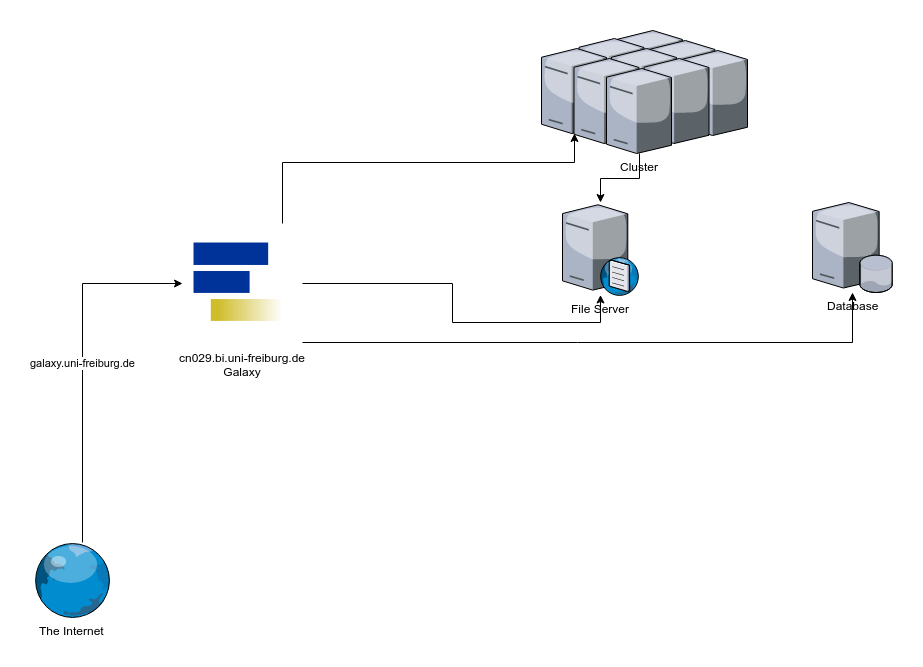
\includegraphics[height=\paperheight,width=\paperwidth]{galaxy-0.png-border.png}}
	\setbeamertemplate{navigation symbols}{}
	\begin{frame}[plain]
	\end{frame}
}
{%
	\usebackgroundtemplate{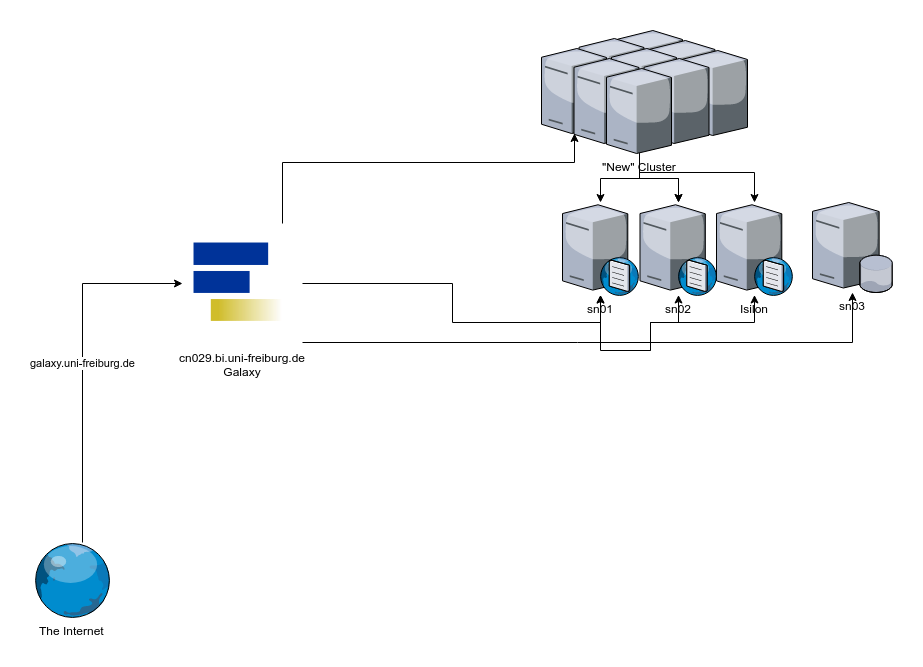
\includegraphics[height=\paperheight,width=\paperwidth]{galaxy-1.png-border.png}}
	\setbeamertemplate{navigation symbols}{}
	\begin{frame}[plain]
	\end{frame}
}
{%
	\usebackgroundtemplate{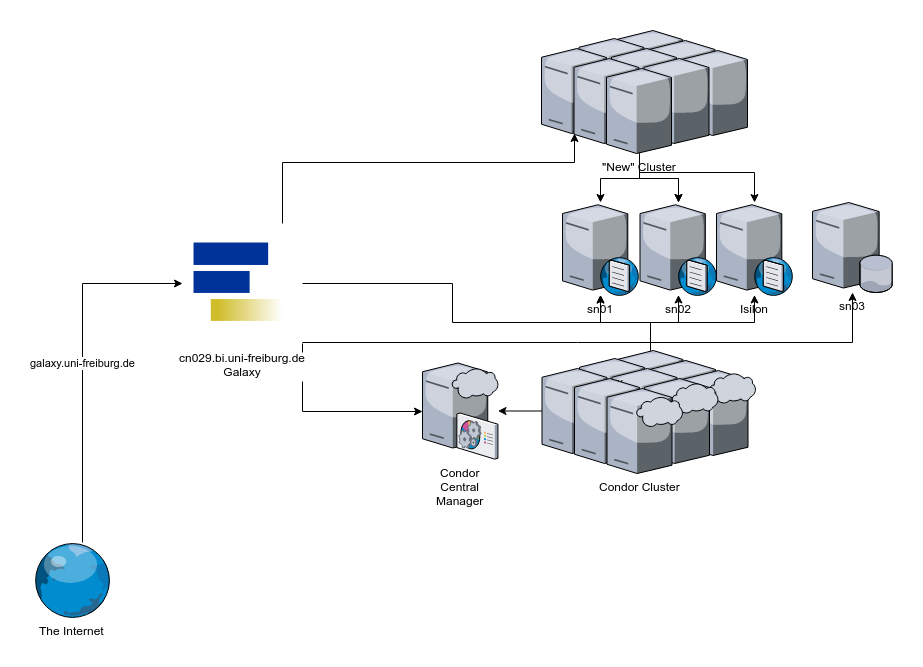
\includegraphics[height=\paperheight,width=\paperwidth]{galaxy-2.png-border.png}}
	\setbeamertemplate{navigation symbols}{}
	\begin{frame}[plain]
	\end{frame}
}
{%
	\usebackgroundtemplate{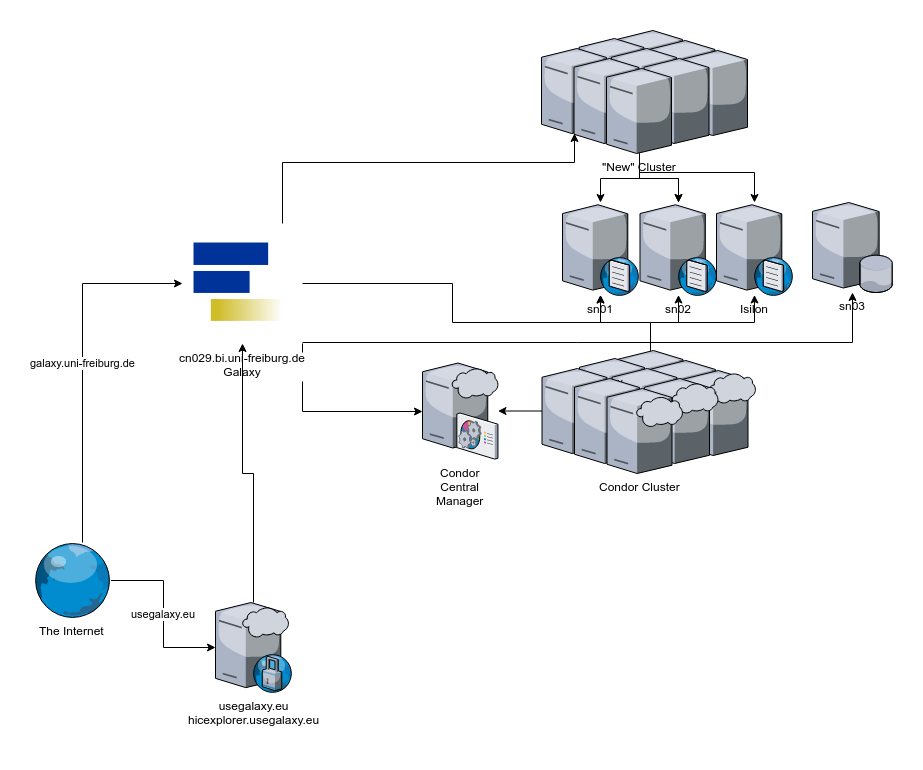
\includegraphics[height=\paperheight,width=\paperwidth]{galaxy-3.png-border.png}}
	\setbeamertemplate{navigation symbols}{}
	\begin{frame}[plain]
	\end{frame}
}
{%
	\usebackgroundtemplate{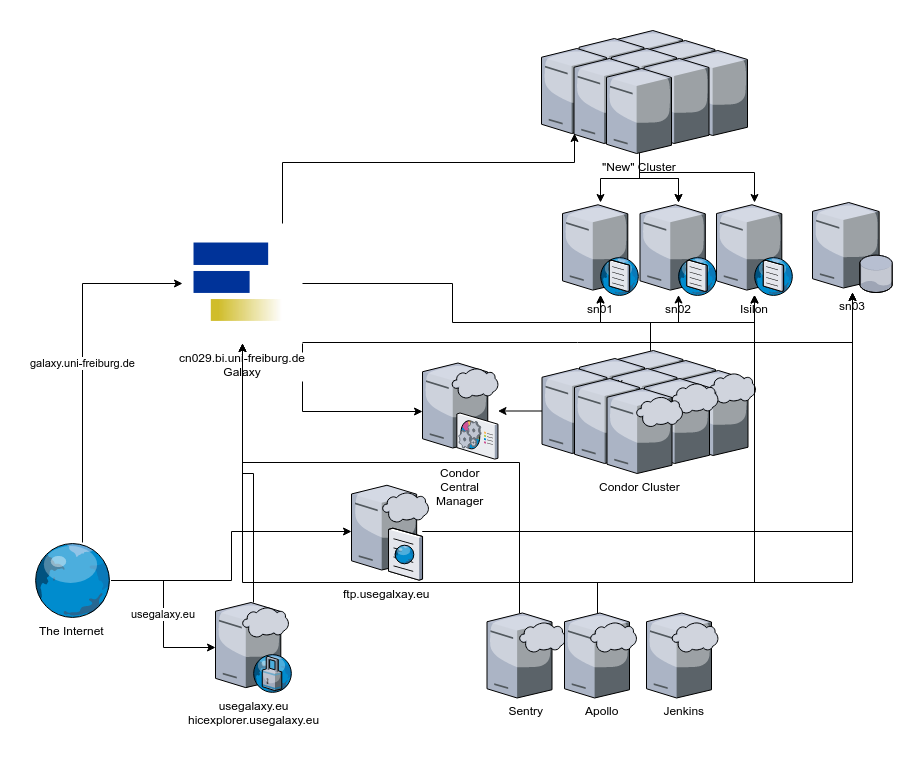
\includegraphics[height=\paperheight,width=\paperwidth]{galaxy-4.png-border.png}}
	\setbeamertemplate{navigation symbols}{}
	\begin{frame}[plain]
	\end{frame}
}
{%
	\usebackgroundtemplate{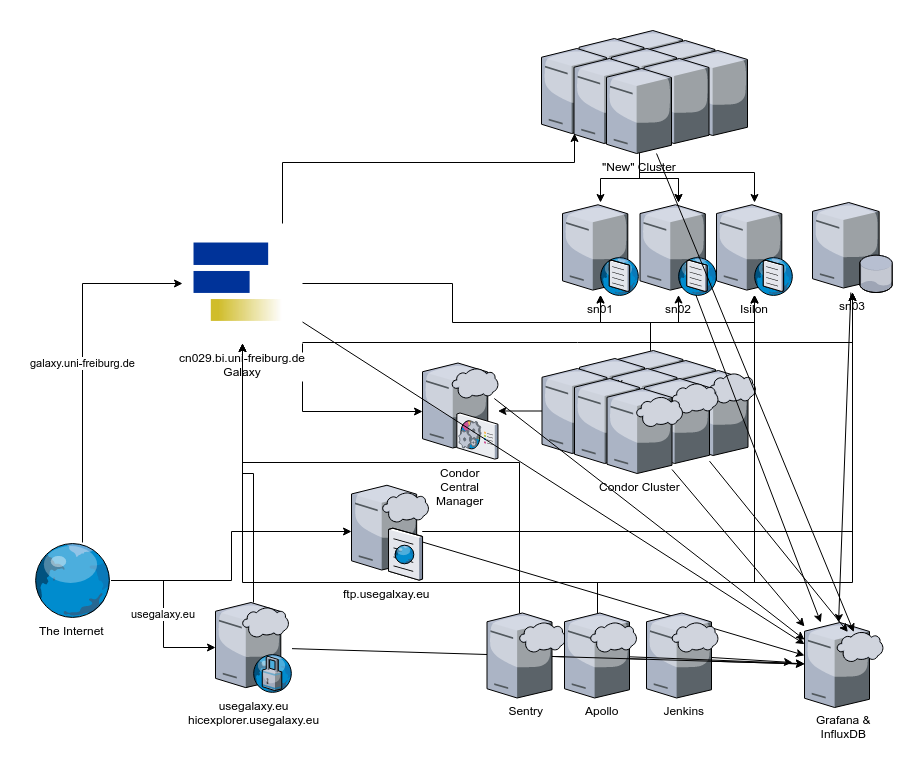
\includegraphics[height=\paperheight,width=\paperwidth]{galaxy-5.png-border.png}}
	\setbeamertemplate{navigation symbols}{}
	\begin{frame}[plain]
	\end{frame}
}
{%
	\usebackgroundtemplate{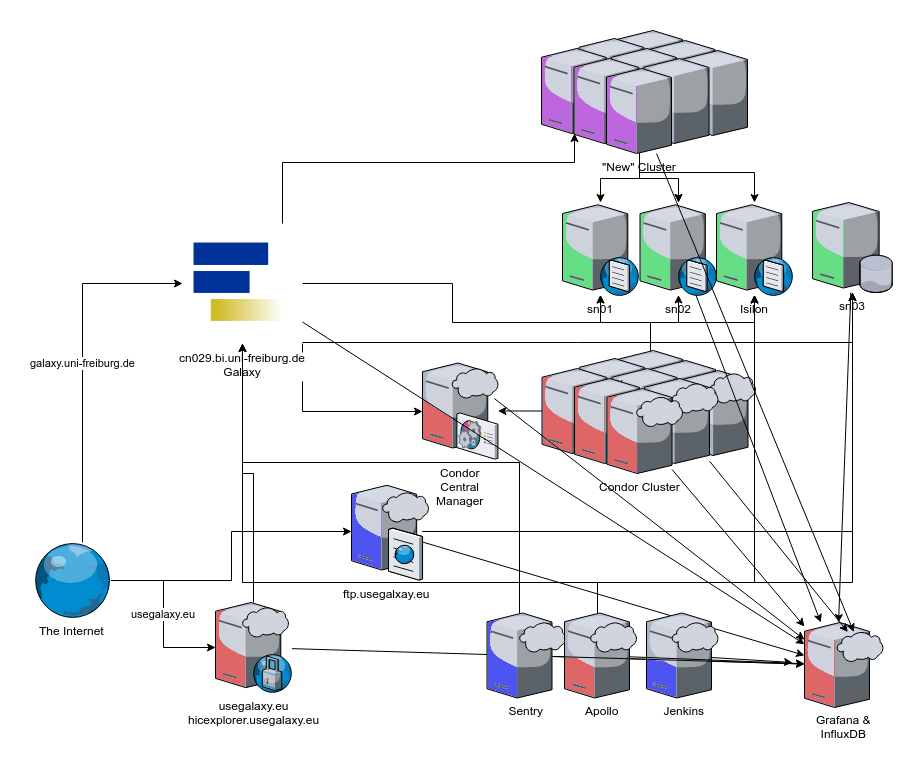
\includegraphics[height=\paperheight,width=\paperwidth]{galaxy-6.png-border.png}}
	\setbeamertemplate{navigation symbols}{}
	\begin{frame}[plain]
	\end{frame}
}
{%
	\usebackgroundtemplate{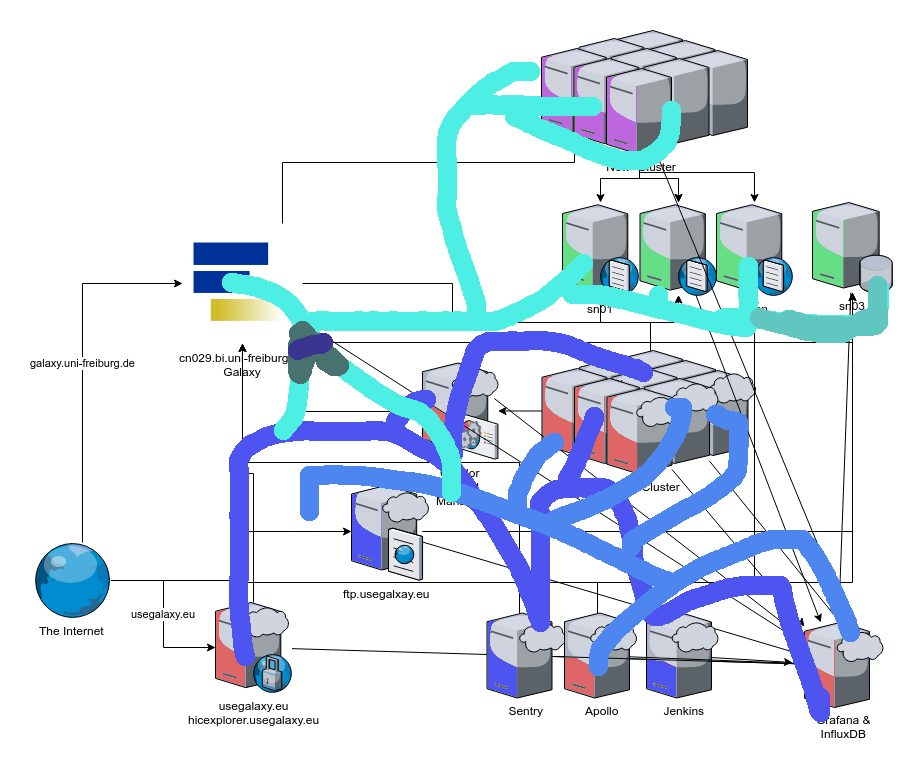
\includegraphics[height=\paperheight,width=\paperwidth]{galaxy-7.png-border.png}}
	\setbeamertemplate{navigation symbols}{}
	\begin{frame}[plain]
	\end{frame}
}

\begin{frame}{Overall System Goals}
	We have to balance the needs of the system:
	\vfill
	\begin{itemize}
		\item Galaxy is up and functioning correctly
		\item Even when things are going wrong
		\item Automatically handle bad situations where possible
		\item Related services are available to users
	\end{itemize}
	\vfill
	\pause
	With our needs:
	\vfill
	\begin{itemize}
		\item We aren't burning out
		\item Work is enjoyable
		\item We feel like we're making a positive impact
		\item We can take holidays
	\end{itemize}
\end{frame}

\begin{frame}{The Humans Behind the Infrastructure}
	We are more than a chatbox in gitter or the voices on the other side of the
	phone.
	\vfill
	\begin{itemize}
		\item We make mistakes
		\item So we have to plan for this and write validation and guards against it
		\item Sometimes problems are bigger than one person's abilities
		\item So we have to work together efficiently and effectively
	\end{itemize}
\end{frame}

\begin{frame}{tl;dr}
	Must balance
	\begin{itemize}
		\item High system uptime (and the engineering required to achieve that)
		\item Manageable amount of work for sysadmins
		\item Guard against sources of error (esp. humans)
	\end{itemize}
\end{frame}

\section{Human Infra}
\begin{frame}{Managing the Insanity}
	Some strategies:
	\begin{itemize}
		\item Standardisation
		\item Bus Factor
		\item KISS
		\item Code defensively
		\item Validate \emph{everything}
		\item Documentation \& Read-Only Fridays
		\item Do not trust the Cloud
		\item Empathy
	\end{itemize}
\end{frame}

\subsection{Standardisation}
\begin{frame}{Standardisation}
	Standard corporate programming attitudes:
	\begin{itemize}
		\item Custom services are written in Python
		\item VMs are based on CentOS 7
		\item \emph{Everything} configured with Ansible
		\item \texttt{Makefile} for everything
	\end{itemize}
\end{frame}

\subsection{Bus Factor}
\begin{frame}{Bus Factor}
	\begin{quote}
		The bus factor is a measurement of the risk resulting from information
		and capabilities not being shared among team members, from the phrase
		``in case they get hit by a bus''.\cite{wiki:Bus_factor}
	\end{quote}
	\vfill
	\begin{itemize}
		\item ``Bus Factor'' is continually a concern
		\item Strategies to decrease:
		\begin{itemize}
			\item Two people responsible per item
			\item Explicitly training + Continual communication of knowledge
			\item \texttt{make} must be accomplish every task
			\item \texttt{make help} explains everything necessary to run it
		\end{itemize}
		%\item Decreases friction when moving between repositories
	\end{itemize}
\end{frame}

\subsection{KISS}
\begin{frame}{Keep It Simple Silly}
	\begin{itemize}
		\item Do you really need another makefile task?
		\item Is this feature needed?
		\item Can I eliminate this code?
		\item Can I simplify this (while avoiding code golf)
		\item \emph{But keep it readable}
	\end{itemize}
	\vfill
	Less I have to think $\Rightarrow$ Less chance for a mistake
\end{frame}

\subsection{Defense}
\begin{frame}{Code Defensively}
	\begin{itemize}
		\item Validate \emph{all} inputs
		\item Do not trust ``trusted'' sources
		\item Timeout all network operations
		\item Retry all network operations
		\item Add jitter\cite{aws:jitter}
	\end{itemize}
	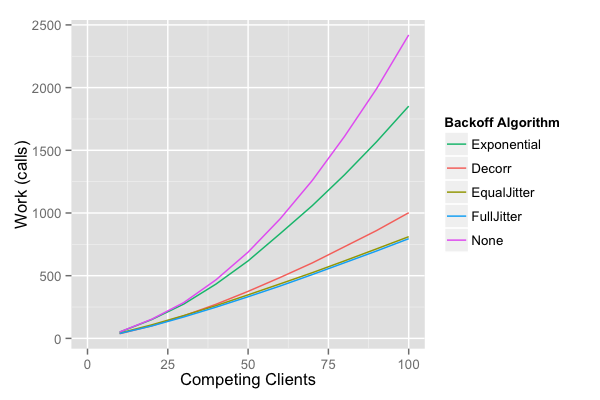
\includegraphics[width=0.5\textwidth]{exponential-backoff-and-jitter-blog-figure-12.png}
\end{frame}

\subsection{Validation}
\begin{frame}{Validate Everything}
	Why:
	\begin{itemize}
		\item It makes life easier
		\item Catch errors before they're live
		\item Better UX for users/devs
	\end{itemize}
	\vfill
	Validate your:
	\begin{itemize}
		\item Configuration files
		\item Code
		\item Datasets
		\item Servers/Functionality
	\end{itemize}
\end{frame}

\subsection{Fridays}
\begin{frame}{Read Only Fridays}
	Do not make changes to production services on friday.

	You will lose your weekend; you will be unhappy
	\vfill
	Instead:
	\begin{itemize}
		\item Document your own code
		\item Document other people's code
		\item Read/test new strategies locally
		\item Simulate failures
	\end{itemize}
\end{frame}

\subsection{Cloud Services}
\begin{frame}{Rules of Cloudland}
	\begin{enumerate}
		\item VMs will go down without warning
		\item VMs can be deleted at any time
		\item Everything is flexible
		\item Nothing is certain%\footnote{but VM death and the Meltdown/Spectre Tax}
	\end{enumerate}
\end{frame}

\begin{frame}{Cloudy With a Chance of Downtime}
	\begin{itemize}
		\item How to handle this uncertainty?
		\item SLA: Service Level Agreement
		\item SLO: Service Level Objectives
			\vfill
			\begin{tabular}{rlll}
				Service        & SLO    & Outage (30d) & User-Facing? \\ \hline
			Haproxy        & 99.9\% & \SI{43}{\minute}   & Yes          \\
			JCaaS          & 99.0\% & \SI{7}{\hour}      & Yes-ish      \\
			FTP            & 95.0\% & \SI{36}{\hour}     & Yes          \\
			Condor Cluster & 95.0\% & \SI{36}{\hour}     & Yes-ish      \\
			Apollo         & 90.0\% & \SI{72}{\hour}     & Yes          \\
			Sentry         & 50.0\% & \SI{15}{\day}      & No           \\
			Jenkins        & 50.0\% & \SI{15}{\day}      & No           \\
			Grafana        & 50.0\% & \SI{15}{\day}      & Yes-ish      \\
			InfluxDB       & 50.0\% & \SI{15}{\day}      & No           \\
			CSP            & 50.0\% & \SI{15}{\day}      & No           \\
		\end{tabular}
	\end{itemize}
\end{frame}


\subsection{Empathy}
\begin{frame}{Empathy}
	\begin{itemize}
		\item Empathy is part of the job
		\item Bad things happen $\Rightarrow$ be kind to each other/ourselves
		%\item We share responsibility; for code, for success, for failure
		%\item Someone else will debug your code at 3am
		\item Small changes affect 100s-1000s of people
		\item Having empathy for users when we break something helps defuse bad situations
	\end{itemize}
\end{frame}


\section{Non-Human Infra}
\begin{frame}{useGalaxy.eu infrastructure}
	Some examples where we've applied these principles to our services and it has helped us.
\end{frame}


\subsection{Haproxy}
\begin{frame}{Haproxy}
	\begin{itemize}
		\item Responds to your requests for \texttt{usegalaxy.eu}
		\item Routes incoming traffic to correct backend
		\item Enables future Galaxy frontend failover
	\end{itemize}
	\vfill
	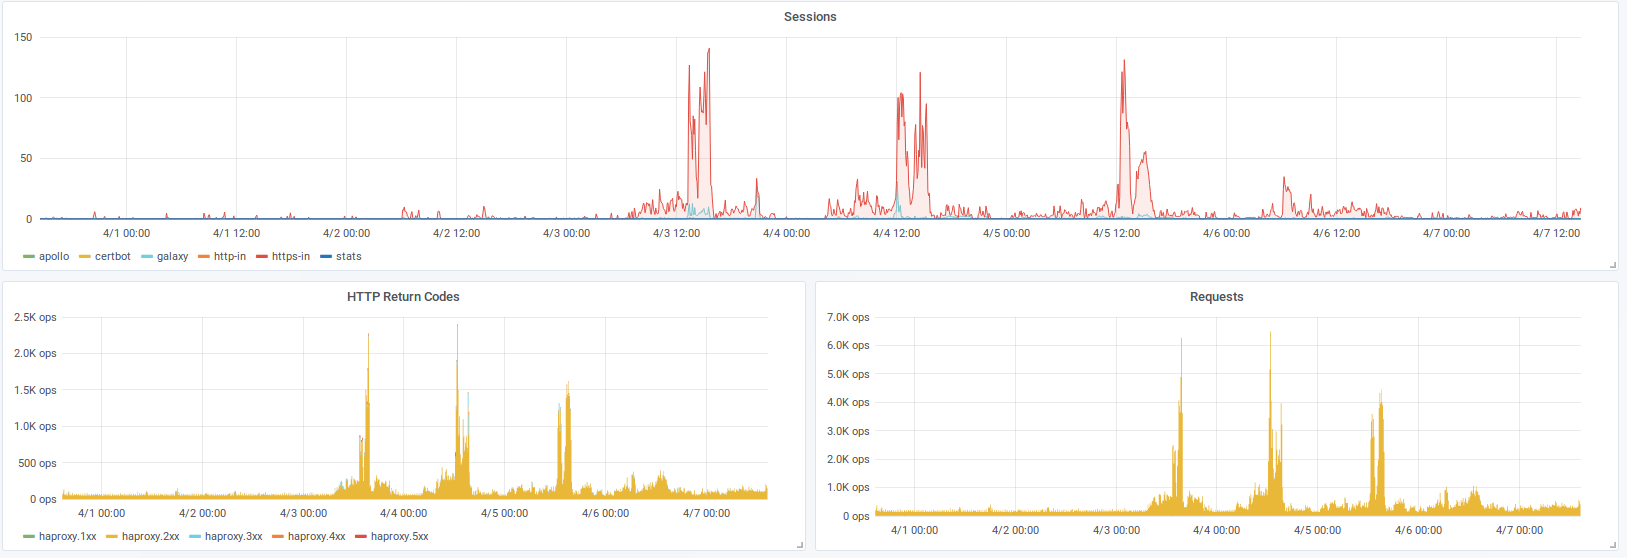
\includegraphics[width=\textwidth]{haproxy.png}
\end{frame}

\subsection{JCaaS}
\begin{frame}{Job Configuration\ldots{}as a Service!}
	\begin{itemize}
		\item Enables Training Infrastructure as a Service
		\item Makes life \emph{so} much easier
		\item Tool destination (memory, CPU cores, environment) changes can take effect without a slow handler restart
		\item Can turn off a mis-behaving cluster instantaneously
	\end{itemize}
\end{frame}

\subsection{FTP}
\begin{frame}{FTP}
	\begin{itemize}
		\item Example of the ideal human-managed service
		\item All state is stored in playbooks or in NFS
		\item When it fails or misbehaves in any way, we can just replace it
	\end{itemize}
\end{frame}

\subsection{Condor Cluster}
\begin{frame}{Condor Cluster}
	\begin{columns}[T] % align columns
		\begin{column}{.48\textwidth}
			\begin{itemize}
				\item Cluster in the Cloud
				\item Easy to roll out new images
				\item Easy for humans to manage
			\end{itemize}
		\end{column}%
		\hfill%
		\begin{column}{.48\textwidth}
			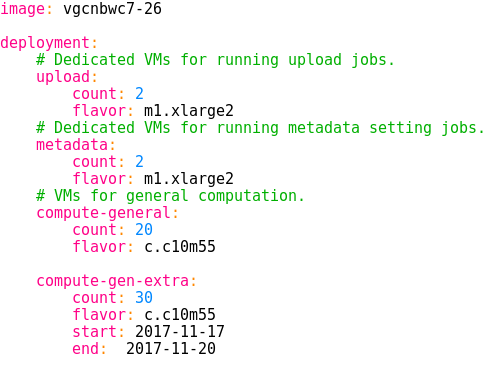
\includegraphics[width=0.9\textwidth]{vgcn-config.png}
		\end{column}%
	\end{columns}

	\vfill
	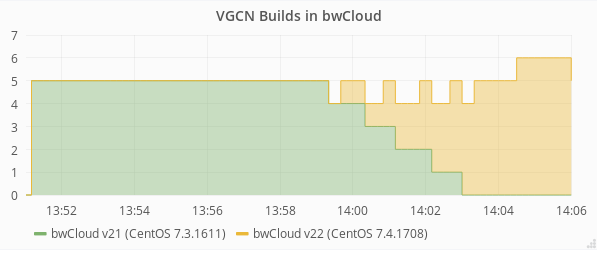
\includegraphics[width=\textwidth]{vgcn.png}
\end{frame}

\section{End}
\begin{frame}{Thank y'all}
Thank \emph{you} for the bug reports and your patience when outages happen.
\vfill
We are doing our best. Don't hesitate to let us know when things aren't working
like expected! Maybe we aren't monitoring it yet.
\vfill
\end{frame}

\section{References}
\begin{frame}[allowframebreaks]
	\frametitle{References}
	\bibliographystyle{plain}
	\bibliography{main.bib}
\end{frame}

\end{document}
